% Szglab4
% ===========================================================================
%
\chapter{Szkeleton tervezése}

\thispagestyle{fancy}

\section{Errata}

Az előző fejezetben leírtak egy apró részletben megváltoztak. Az elemeket már nem közvetlenül kötjük össze, hanem \textit{vezeték}ek segítségével, melyeket egymással \textit{csomópont}okkal lehet összekötni, ha szükséges. Így javítottuk a láthatósággal kapcsolatosan felmerült problémákat, ehhez fel kellett venni 2 új osztályt (Wire, Node), illetve az AbstractComponent módosítani, ezekhez tartozó objektum és osztályleírások alább olvashatóak, valamint mellékeltük a módosított statikus osztálydiagramot is. (Egy-két egyéb objektumleírás is módosult, de csak azért mert a kiértékelés logikája változott -- nem hátulról megyünk, hanem az összes kiértékeli magát, ez nem szükséges a jelen fejezethez, hiszen magától értetődő)

\subsection{Objektumleírás: \bf Wire}
Vezeték, mely az áramköri komponensek ki és bemeneteit köti össze. Egy vezeték egy darab kimenetet és egy darab bemenetet köt össze. A rajta lévő értéket le lehet tőle kérdezni, illetve be lehet azt állítani.

\subsection{Objektumleírás: \bf Node}
Csomópont, mely a bemenetén lévő értéket a kimeneteire adja. Segítségével lehet egy vezetéket ,,szétágaztatni''.

\subsection{Osztályleírás: \bf AbstractComponent}
Absztrakt osztály.
\begin{itemize}
\item Felelősség\\
Egy komponens absztrakt megvalósítása, ebből származik az összes többi  komponens. A közös logikát valósítja meg. A gyakran használt feladatokra ad alapértelmezett implementációt (pl. vezetékek bekötése). Tudja magáról, hogy a legutóbbi két kiértékelés között változtak-e a kimenetei.
\item Ősosztályok: (nincs)
\item Interfészek: (nincs)
\item Attribútumok $\ $
\begin{itemize}
	\item \texttt{protected Wire[] inputs}: Bemeneteire kötött vezetékek.
	\item \texttt{protected Wire[] outputs}: Kimeneteire kötött vezetékek.
\end{itemize}
\item Metódusok$\ $
\begin{itemize}
	\item \texttt{addTo(Circuit c)}: Meghívja az áramkör \texttt{add(AbstractComponent ac)} metódusát.
	\item \texttt{void evaluate()}: Komponens kimenetein lévő értékek kiszámolása a bemenetek alapján.
	\item \texttt{boolean isChanged()}: Visszaadja, hogy a legutóbbi két kiértékelés között változtak-e a kimenetek.
	\item \texttt{void setInput(int inputPin, Wire wire)}: Az adott bemeneti lábára rákötjük a megadott vezetéket.
	\item \texttt{void setOutput(int outputPin, Wire wire)}: Az adott kimeneti lábára rákötjük a megadott vezetéket.
\end{itemize}
\end{itemize}

\subsection{Osztályleírás: \bf Node}
\begin{itemize}
\item Felelősség\\
Csomópont, mely a bemenetén lévő értéket a kimeneteire adja. Segítségével lehet egy vezetéket ,,szétágaztatni''.
\item Ősosztályok:\ AbstractComponent.
\item Interfészek: (nincs)
\item Attribútumok $\ $
\begin{itemize}
\item (nincs)
\end{itemize}
\item Metódusok$\ $
\begin{itemize}
\item (nincs)
\end{itemize}
\end{itemize}

\subsection{Osztályleírás: \bf Wire}
\begin{itemize}
\item Felelősség\\
Vezeték, mely az áramköri komponensek ki és bemeneteit köti össze. Egy vezeték egy darab kimenetet és egy darab bemenetet köt össze. A rajta lévő értéket le lehet tőle kérdezni, illetve be lehet azt állítani.
\item Ősosztályok:\ AbstractComponent.
\item Interfészek: (nincs)
\item Attribútumok $\ $
\begin{itemize}
	\item \texttt{private Value value}: Vezetéken lévő érték
\end{itemize}
\item Metódusok$\ $
\begin{itemize}
	\item \texttt{Value getValue()}: Visszaadja a vezetéken lévő értéket.
	\item \texttt{void settValue(Value v)}: Beállítja a vezetéken lévő értéket.
\end{itemize}
\end{itemize}

\subsection{Statikus struktúra diagramok}

\begin{figure}[H]
\begin{center}
\includegraphics*[angle=90, width=17cm, viewport = 25 30 705 565]{chapters/chapter04/classdiagram/class.pdf}
\caption{Statikus struktúra nézet}
\label{fig:class_diagram}
\end{center}
\end{figure}

\section{A szkeleton modell valóságos use-case-ei}

\subsection{Use-case diagram}

\begin{figure}[h]
\begin{center}
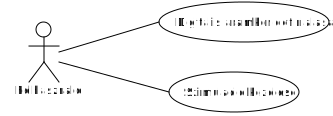
\includegraphics[width=10cm]{chapters/chapter05/imgs/usecase.pdf}
\caption{A szkeleton modell valóságos use-case-ei}
\label{fig:SzkeletonUseCase}
\end{center}
\end{figure}

\subsection{Use-case leírások}

\usecase
{Áramkör inicializálása}
{Ez a usecase egy áramkör és a hozzá tartozó szimuláció inicializálását mutatja be, hogyan jönnek létre a komponensek és a közöttük lévő összeköttetés. Jelen példa egy Kapcsoló és egy Led összeköttetését prezentálja.}
{Tesztelő}
{\vspace{-15pt}
\begin{itemize}
\setlength{\itemsep}{0cm}%
\setlength{\parskip}{0cm}%
\item szimuláció létrehozása
\item áramkör létrehozása
\item áramkör beregisztrálása a szimulációba
\item áramkör inicializálása
\begin{itemize}
\setlength{\itemsep}{0cm}%
\setlength{\parskip}{0cm}%
	\item kapcsoló létrehozása
	\item vezeték létrehozása
	\item kapcsoló kimenetére vezeték kötése
	\item led létrehozása
	\item led bemenetére vezeték kötése
	\item kapcsoló áramkörbe regisztrálása
	\item led áramkörbe regisztrálása
\end{itemize}
\end{itemize}
\vspace{-15pt}}

\usecase
{Kapcsoló és Led}
{Ez a usecase egy olyan áramkör tesztelését mutatja be, amely egy kapcsolóból és rá kötött ledből áll.}
{Tesztelő}
{\vspace{-15pt}
\begin{itemize}
\setlength{\itemsep}{0cm}%
\setlength{\parskip}{0cm}%
\item Áramkör és komponensek létrehozása
%\begin{itemize}
%\setlength{\itemsep}{0cm}%
%\setlength{\parskip}{0cm}%
%\item áramkör létrehozása
%\item áramkör beregisztrálása a szimulációba
%\item vezeték létrehozása
%\item kapcsoló létrehozása
%\item kapcsoló kimenetére vezeték kötése
%\item led létrehozása
%\item led bemenetére vezeték kötése
%\item kapcsoló áramkörbe regisztrálása
%\item led áramkörbe regisztrálása
%\end{itemize}
\item kapcsoló értékének beállítása (\textbf{megkérdezi a tesztelőt})
\item szimuláció indítása
\begin{itemize}
\setlength{\itemsep}{0cm}%
\setlength{\parskip}{0cm}%
\item hálózat kiértékelés indítása
\begin{itemize}
\setlength{\itemsep}{0cm}%
\setlength{\parskip}{0cm}%
\item kapcsoló kiértékelése (állapotának kijelzése)
\item led kiértékelése (világít/nem világít kijelzése)
\end{itemize}
\item áramkör változásának vizsgálata
\item stacionárius állapot, szimuláció vége
\end{itemize}
\end{itemize}
\vspace{-15pt}}

\usecase
{Kapcsoló, Inverter és Led}
{Ez a usecase egy olyan áramkör tesztelését mutatja be, amely egy kapcsolóból egy rá kötött inverterből és egy arra kötött ledből áll.}
{Tesztelő}
{\vspace{-15pt}
\begin{itemize}
\setlength{\itemsep}{0cm}%
\setlength{\parskip}{0cm}%
\item Áramkör és komponensek létrehozása
%\begin{itemize}
%\setlength{\itemsep}{0cm}%
%\setlength{\parskip}{0cm}%
%\item áramkör létrehozása
%\item áramkör beregisztrálása a szimulációba
%\item vezeték létrehozása a kapcsoló és az inverter összekötéséhez
%\item kapcsoló létrehozása
%\item kapcsoló kimenetére vezeték kötése
%\item inverter létrehozása
%\item inverter bemenetére vezeték kötése
%\item vezeték lérehozása az inverter és a led összekötéséhez
%\item inverter kimenetére vezeték kötése
%\item led létrehozása
%\item led bemenetére vezeték kötése
%\item kapcsoló áramkörhöz adása
%\item led áramkörhöz adása
%\item inverter áramkörhöz adása
%\end{itemize}
\item kapcsoló értékének beállítása (\textbf{megkérdezi a tesztelőt})
\item szimuláció indítása
\begin{itemize}
\setlength{\itemsep}{0cm}%
\setlength{\parskip}{0cm}%
\item hálózat kiértékelés indítása (2x)
\begin{itemize}
\setlength{\itemsep}{0cm}%
\setlength{\parskip}{0cm}%
\item kapcsoló kiértékelése (állapotának kijelzése)
\item inverter kiértékelése
\begin{itemize}
\setlength{\itemsep}{0cm}%
\setlength{\parskip}{0cm}%
\item bemenetén lévő érték lekérése
\item kimenetére kötött érték kiszámolása és kiadása
\end{itemize}
\item led kiértékelése (világít/nem világít kijelzése)
\end{itemize}
\item áramkör változásának vizsgálata
\item két lépés alatt stacionárius állapot\footnote{amennyiben a kapcsoló logikai igazra van állítva, akkor egy lépés is elég, de két lépés biztosan, így ezt ábrázoljuk diagramon}, szimuláció vége
\end{itemize}
\end{itemize}
\vspace{-15pt}}

\usecase
{2 Kapcsoló, Vagy kapu és Led}
{Ez a usecase egy olyan áramkör tesztelését mutatja be, amely egy vagy kapura kötött két kapcsolóból és a vagy kapu kimenetére kötött ledből áll.}
{Tesztelő}
{\vspace{-15pt}
\begin{itemize}
\setlength{\itemsep}{0cm}%
\setlength{\parskip}{0cm}%
\item Áramkör és komponensek létrehozása
%\begin{itemize}
%\setlength{\itemsep}{0cm}%
%\setlength{\parskip}{0cm}%
%\item áramkör létrehozása
%\item áramkör beregisztrálása a szimulációba
%\item vezeték létrehozása az egyik kapcsoló és a vagy kapu összekötéséhez
%\item egyik kapcsoló létrehozása
%\item kapcsoló kimenetére vezeték kötése
%\item vezeték létrehozása a másik kapcsoló és a vagy kapu összekötéséhez
%\item másik kapcsoló létrehozása
%\item kapcsoló kimenetére vezeték kötése
%\item VAGY kapu létrehozása
%\item VAGY kapu bemeneteire a fenti két vezeték kötése
%\item vezeték létrehozása a vagy kapu és a led összekötéséhez
%\item VAGY kapu kimenetére vezeték kötése
%\item led létrehozása
%\item led bemenetére vezeték kötése
%\item kapcsolók áramkörhöz adása
%\item VAGY kapu áramkörhöz adása
%\item led áramkörhöz adása
%\end{itemize}
\item egyik kapcsoló értékének beállítása (\textbf{megkérdezi a tesztelőt})
\item másik kapcsoló értékének beállítása (\textbf{megkérdezi a tesztelőt})
\item szimuláció indítása
\begin{itemize}
\setlength{\itemsep}{0cm}%
\setlength{\parskip}{0cm}%
\item hálózat kiértékelés indítása (2x)
\begin{itemize}
\setlength{\itemsep}{0cm}%
\setlength{\parskip}{0cm}%
\item egyik kapcsoló kiértékelése (állapotának kijelzése)
\item másik kapcsoló kiértékelése (állapotának kijelzése)
\item VAGY kapu kiértékelése
\begin{itemize}
\setlength{\itemsep}{0cm}%
\setlength{\parskip}{0cm}%
\item bemenetén lévő értékek lekérése
\item kimenetére kötött érték kiszámolása és kiadása
\end{itemize}
\item led kiértékelése (világít/nem világít kijelzése)
\end{itemize}
\item áramkör változásának vizsgálata
\item második lépés után stacionárius állapot\footnote{amennyiben mindkét kapcsoló 0-ás állapotban van, egy lépés alatt stabil lesz a hálózat, hiszen a VAGY kapu végig hamis állapotot ad ki, itt és a szekvencia diagramon úgy vesszük, mintha legalább az egyik kapcsoló 1-esbe lenne állítva.}, szimuláció vége
\end{itemize}
\end{itemize}
\vspace{-15pt}}

\newpage

\usecase
{Inverter visszakötve és Led}
{Ez a usecase egy olyan áramkör tesztelését mutatja be, amely egy inverterből, amelynek kimenete egy ledbe illetve saját bemenetére van kötve. Oszcillálni fog, ezért a szimuláció rövid időn belül leáll.}
{Tesztelő}
{\vspace{-15pt}
\begin{itemize}
\setlength{\itemsep}{0cm}%
\setlength{\parskip}{0cm}%
\item Áramkör és komponensek létrehozása
%\begin{itemize}
%\setlength{\itemsep}{0cm}%
%\setlength{\parskip}{0cm}%
%\item áramkör létrehozása
%\item áramkör beregisztrálása a szimulációba
%\item inverter létrehozása
%\item vezeték létrehozása az inverter és a csomópont összekötéséhez
%\item inverter kimenetére vezeték kötése
%\item csomópont létrehozása
%\item csomópont bemenetére vezeték kötése
%\item vezeték létrehozása a csomópont és az inverter (bemenetre) összekötéséhez
%\item csomópont egyik kimenetére vezeték kötése
%\item inverter bemenetére vezeték kötése
%\item vezeték létrehozása a csomópont és a led összekötéséhez
%\item csomópont másik kimenetére vezeték kötése
%\item led létrehozása
%\item led bemenetére vezeték kötése
%\item inverter áramkörhöz adása
%\item led áramkörhöz adása
%\end{itemize}
\item szimuláció indítása
\begin{itemize}
\setlength{\itemsep}{0cm}%
\setlength{\parskip}{0cm}%
\item hálózat kiértékelés indítása (3x)
\begin{itemize}
\setlength{\itemsep}{0cm}%
\setlength{\parskip}{0cm}%
\item inverter kiértékelése
\begin{itemize}
\setlength{\itemsep}{0cm}%
\setlength{\parskip}{0cm}%
\item bemenetén lévő értékek lekérése
\item kimenetére kötött érték kiszámolása és kiadása
\end{itemize}
\item csomópont kiértékelése
\begin{itemize}
\setlength{\itemsep}{0cm}%
\setlength{\parskip}{0cm}%
\item bemenetén lévő érték lekérése
\item kimeneteire az érték kiadása
\end{itemize}
\item led kiértékelése (világít/nem világít kijelzése)
\end{itemize}
\item áramkör változásának vizsgálata
\item harmadik lépés után sincs stacionárius állapot, szimuláció vége
\end{itemize}
\end{itemize}
\vspace{-15pt}}

\usecase
{Kapcsoló, Vagy kapu visszakötve és Led}
{Ez a usecase egy olyan áramkör tesztelését mutatja be, amely egy kapcsolóból, egy VAGY kapuból, melynek egyik bemenetére a kapcsoló, másik bemenetére a saját kimenete van kötve és egy ledből, melyre szintén a VAGY kapu kimenetét kötöttük. Ez egy olyan visszakötéses hálózat, mely stabil állapotban van.}
{Tesztelő}
{\vspace{-15pt}
\begin{itemize}
\setlength{\itemsep}{0cm}%
\setlength{\parskip}{0cm}%
\item Áramkör és komponensek létrehozása
%\begin{itemize}
%\setlength{\itemsep}{0cm}%
%\setlength{\parskip}{0cm}%
%\item áramkör létrehozása
%\item áramkör beregisztrálása a szimulációba
%\item kapcsoló létrehozása
%\item vezeték létrehozása a kapcsoló és a VAGY kapu összekötéséhez
%\item kapcsoló kimenetére vezeték kötése
%\item VAGY kapu létrehozása
%\item VAGY kapu egyik bemenetére vezeték kötése
%\item vezeték létrehozása a VAGY kapu és a csomópont összekötéséhez
%\item VAGY kapu kimenetére vezeték kötése
%\item csomópont létrehozása
%\item csomópont bemenetére vezeték kötése
%\item vezeték létrehozása a csomópont és a vagy kapu (bemenetének) összekötéséhez
%\item csomópont egyik kimenetére vezeték kötése
%\item VAGY kapu másik bemenetére vezeték kötése
%\item vezeték létrehozása a csomópont és a led összekötéséhez
%\item csomópont másik kimenetére vezeték kötése
%\item led létrehozása
%\item led bemenetére vezeték kötése
%\item kapcsoló áramkörhöz adása
%\item VAGY kapu áramkörhöz adása
%\item led áramkörhöz adása
%\end{itemize}
\item szimuláció indítása
\begin{itemize}
\setlength{\itemsep}{0cm}%
\setlength{\parskip}{0cm}%
\item hálózat kiértékelés indítása (2x)
\begin{itemize}
\setlength{\itemsep}{0cm}%
\setlength{\parskip}{0cm}%
\item kapcsoló kiértékelése (állapotának kijelzése)
\item VAGY kapu kiértékelése
\begin{itemize}
\setlength{\itemsep}{0cm}%
\setlength{\parskip}{0cm}%
\item bemenetén lévő értékek lekérése
\item kimenetére kötött érték kiszámolása és kiadása
\end{itemize}
\item csomópont kiértékelése
\begin{itemize}
\setlength{\itemsep}{0cm}%
\setlength{\parskip}{0cm}%
\item bemenetén lévő érték lekérése
\item kimeneteire az érték kiadása
\end{itemize}
\item led kiértékelése (világít/nem világít kijelzése)
\end{itemize}
\item áramkör változásának vizsgálata
\item második lépés után stacionárius állapot\footnote{ha a kapcsoló 0-ás állapotban van, akkor egy lépés alatt bekövetkezik, de érdekesebb szituáció, amikor 1-es állapotban van, ezt ábrázoljuk diagramon}, szimuláció vége
\end{itemize}
\end{itemize}
\vspace{-15pt}}

\section{Architektúra}

\section{A szkeleton kezelői felületének terve, dialógusok}
%\comment{A szkeleton által elfogadott bemenetek , valamint a szöveges konzolon megjelenő kimenetek. A %kiemenet formátuma olyan kell legyen, ami alapján a működés összevethető a korábbi szekvencia-%
%diagramokkal.}
Az általunk elkészített szkeleton egy  program váz melynek felülete egy egyszerű konzolos megjelenítési felület, amely alkalmas arra, hogy a use case-k által leírt teszteseteket bemutassuk. Az egyes tesztesetek a neki megfelelő use case sorszámával van elnevezve, így program indítás után egy szám bevitelét követően a kiválasztott teszteset lefut. 
A teszteset futása közben kiír minden objektumot amin metódust hív, illetve kiírja a metódus nevét a paraméterekkel együtt, majd a visszatérési értéket. Ez azért lehetséges, mert a szkeleton már tartalmazza az elkészítendő szoftver összes fontos osztályát és metódusát, azonban az üzleti logikát még nem. Így könnyen eldönthető, hogy a use case-nek megfelelően viselkedik a program és továbbiakban képes lesz-e megfelelően működni.
A tesztelési folyamat során döntési helyzet léphet fel. Ilyenkor a program felteszi a kérdést, majd a kapott válasz alapján folytatja a további futást. Ezzel csökkentjük a tesztesetek számát, anélkül, hogy bizonyos esetek kimaradnának a tesztelés alól. 
Futás közben megjegyzés formájában a program tájékoztat néhány elem belső állapotáról (például kapcsoló értéke) vagy bizonyos fontosabb lépésekről (például inicializálás).
Az elvárás, hogy a szkeleton a szekvenciadiagramok által leírt működést mutassa. A program egyszerű és könnyen összehasonlítható formában írja ki a működését, amelyet könnyen összevethetjük a szekvencia diagrammokkal.

Egy metódushívás és visszatérés esetén kiírt adatok a következők:
\begin{itemize}
\item Metódushívás esetén a CALL szót, konstruktorhívás esetén CREATE szót, míg visszatéréskor a RETURN szót
\item Objektum neve
\item A metódus neve és a metódus paramétereinek értékét
\item Visszatérés esetén a visszatérési értéket
\end{itemize}
 
Egy döntési helyzetben a kiírt adatok a következő:
\begin{itemize}
\item QUESTION szó
\item objektum neve
\item Egy rövid magyarázó szöveg
\item Szögletes zárójelben a lehetséges válaszok
\end{itemize}

Formátumra példa:


\begin{verbatim}
CALL simulation.start()
  CALL circuit.doEvaluationCycle()
    CALL toggle.evaluate()
      QUESTION toggle állapot? [0/1]
1
      CALL toggle_to_inv.setValue(Value.TRUE)
      RETURN
    RETURN
    CALL inv.evaluate()
      CALL toggle_to_inv.getValue()
        QUESTION toggle_to_inv vezetéken lévő érték? [0/1]
1
      RETURN Value.TRUE
      CALL inv_to_led.setValue(Value.FALSE)
      RETURN
    RETURN
    CALL led.evaluate()
      CALL inv_to_led.getValue()
        QUESTION inv_to_led vezetéken lévő érték? [0/1]
0
      RETURN Value.FALSE
      # nem világít
    RETURN
  RETURN
  CALL circuit.doEvaluationCycle()
    CALL toggle.evaluate()
      QUESTION toggle állapot? [0/1]
1
      CALL toggle_to_inv.setValue(Value.TRUE)
      RETURN
    RETURN
    CALL inv.evaluate()
      CALL toggle_to_inv.getValue()
        QUESTION toggle_to_inv vezetéken lévő érték? [0/1]
1
      RETURN Value.TRUE
      CALL inv_to_led.setValue(Value.FALSE)
      RETURN
    RETURN
    CALL led.evaluate()
      CALL inv_to_led.getValue()
        QUESTION inv_to_led vezetéken lévő érték? [0/1]
0
      RETURN Value.FALSE
      # nem világít
    RETURN
  RETURN
  CALL circuit.isChanged()
    CALL toggle.isChanged()
      QUESTION toggle változott? [0/1]
0
    RETURN false
    CALL inv.isChanged()
      QUESTION inv változott? [0/1]
0
    RETURN false
    CALL led.isChanged()
      QUESTION led változott? [0/1]
0
    RETURN false
  RETURN false
RETURN true


\end{verbatim}

\section{Szekvencia diagramok a belső működésre}
\comment{A szkeletonban implementált szekvenciadiagramok. Tipikusan egy use-case egy diagram. Ezek megegyezhetnek a korábban specifikált diagramokkal, de az egyes életvonalakat (lifeline) egyértelműen a szkeletonban példányosított objektumokhoz kell tudni kötni. Azt kell megjeleníteni, hogy a szkeletonban létrehozott objektumok egymással hogyan fognak kommunikálni.}

\begin{figure}[H]
\begin{center}
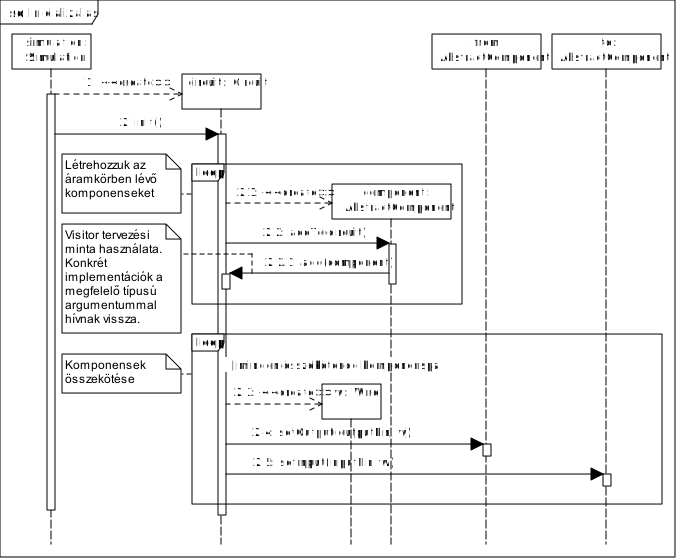
\includegraphics[width=17cm]{chapters/chapter05/imgs/init.pdf}
\caption{Áramkör inicializálása}
\label{fig:init}
\end{center}
\end{figure}

\begin{figure}[H]
\begin{center}
\includegraphics[width=17cm]{chapters/chapter05/imgs/test1.pdf}
\caption{Kapcsoló és Led}
\label{fig:init}
\end{center}
\end{figure}

\begin{figure}[H]
\begin{center}
\includegraphics[angle=90,width=15cm]{chapters/chapter05/imgs/test5.pdf}
\caption{5-ös}
\label{fig:init}
\end{center}
\end{figure}
